\documentclass[journal, a4paper]{IEEEtran}
\usepackage[utf8]{inputenc}
\usepackage[spanish]{babel}
\usepackage{amsmath}
\usepackage{graphicx}
\usepackage{booktabs}
\usepackage{hyperref}
\usepackage{float}

\title{Pre-informe Práctica 0: Manejo de Equipos de Medición en Electrónica Análoga}
\author{
    \textit{jutobara@unal.edu.co} \and
    Juan José Tobar Álvarez\\ \textit{dmontesr@unal.edu.co} \and
    David Alejandro Montes Rodríguez\\ \textit{correo2@unal.edu.co} \and
    Estudiante 3\\ 
}

\begin{document}
\maketitle

\section{Introducción y Justificación}

\subsection{Introducción}
La presente práctica tiene como objetivo capacitar a los estudiantes en el manejo adecuado de los equipos fundamentales de medición en electrónica análoga: el generador de señales, el osciloscopio digital de doble canal y el multímetro digital \cite{guia_practica0}. Durante el desarrollo del laboratorio se aplicarán conceptos de medición de impedancias de entrada y de salida, tensiones eficaces (RMS) y continuas (DC), y potencia disipada; evaluando el comportamiento de estos instrumentos ante señales sinusoidales, cuadradas y triangulares \cite{sedra2020}.

\subsection{Justificación}
El correcto manejo de los instrumentos de medición no es únicamente un requisito académico que se limite a la materia de electrónica análoga, sino que también es una habilidad crítica en la industria tecnológica: una medición inexacta del valor RMS, del nivel DC o de la impedancia de carga puede traducirse en un mal diseño y consecuentemente en el fallo prematuro de un circuito. 

Uno de los sectores industriales en los que la precisión de las medidas se vuelve crítica es el sector aeroespacial. Los osciloscopios se emplean para verificar la integridad de señal de sistemas de radar, comunicaciones y buses de datos como el MIL-STD-1553, permitiendo a los técnicos identificar fallas antes de que comprometan la operación de una aeronave \cite{militaryaerospace_scopes,pilotjohn_scopes}. De manera similar, en la industria médica, los osciloscopios combinados con preamplificadores diferenciales de bajo ruido permiten capturar señales del orden de microvoltios (como las registradas en electrocardiogramas) separándolas del ruido generado por el entorno \cite{tektronix_biomedical}. Estos casos evidencian que dominar el manejo de estos equipos es indispensable para el diseño de sistemas confiables en la vida real.

\section{Cálculos}

\subsection{Análisis del Circuito Resistivo DC}
Para el circuito propuesto en la guía de laboratorio (Fig. 1 de \cite{guia_practica0}), se calculan las tensiones, corrientes y potencias disipadas aplicando las leyes de Kirchhoff y Ohm \cite{sedra2020}. Dado que $V_1 = 5\text{ V}$, $R_1=1\text{ k}\Omega$, $R_2=2.2\text{ k}\Omega$, $R_3=2.2\text{ k}\Omega$ y $R_4=1\text{ k}\Omega$, se determinan primero las resistencias equivalentes. La rama derecha ($R_2$ en serie con $R_4$) es:
\begin{equation}
    R_{eq,24} = R_2 + R_4 = 3.2\text{ k}\Omega
\end{equation}
Esta rama está en paralelo con $R_3$, de modo que la resistencia vista desde el nodo N2 hacia tierra es:
\begin{equation}
    R_{eq,324} = \frac{R_3 \cdot R_{eq,24}}{R_3 + R_{eq,24}} = \frac{2.2\text{k} \cdot 3.2\text{k}}{5.4\text{k}} \approx 1.3037\text{ k}\Omega
\end{equation}
La resistencia total vista por la fuente es $R_T = R_1 + R_{eq,324} \approx 2.3037\text{ k}\Omega$. Por Ley de Ohm, la corriente total entregada por la fuente es:
\begin{equation}
    I_{R1} = \frac{V_1}{R_T} = \frac{5\text{ V}}{2.3037\text{ k}\Omega} \approx 2.170\text{ mA}
\end{equation}
Con este resultado se obtienen las demás tensiones y corrientes del circuito:
\begin{itemize}
    \item $V_{R1} = I_{R1} \cdot R_1 \approx 2.170\text{ V}$
    \item $V_{N2} = V_1 - V_{R1} = 5\text{ V} - 2.170\text{ V} = 2.830\text{ V}$
    \item $I_{R3} = \dfrac{V_{N2}}{R_3} = \dfrac{2.830\text{ V}}{2.2\text{ k}\Omega} \approx 1.286\text{ mA}$
    \item $I_{R2} = I_{R4} = \dfrac{V_{N2}}{R_{eq,24}} = \dfrac{2.830\text{ V}}{3.2\text{ k}\Omega} \approx 0.884\text{ mA}$
    \item $V_{R2} = I_{R2} \cdot R_2 \approx 1.945\text{ V}$
    \item $V_{R4} = I_{R4} \cdot R_4 \approx 0.884\text{ V}$
\end{itemize}
La potencia disipada por cada resistencia ($P = V \cdot I$) se resume en la Tabla \ref{tab:potencias}.

\begin{table}[htbp]
\centering
\caption{Potencia disipada teórica en cada resistencia}
\label{tab:potencias}
\begin{tabular}{@{}lcccc@{}}
\toprule
\textbf{Elemento} & $R_1$ & $R_2$ & $R_3$ & $R_4$ \\ \midrule
$P$ (mW) & 4.710 & 1.719 & 3.639 & 0.781 \\ \bottomrule
\end{tabular}
\end{table}

\subsection{Cálculos Analíticos de Señales AC}
El valor medio ($V_{DC}$) y el valor eficaz ($V_{RMS}$) de una señal periódica $v(t)$ de periodo $T$ se definen como \cite{sedra2020}:
\begin{equation}
    V_{DC} = \frac{1}{T}\int_{0}^{T} v(t)\,dt \: ; \quad V_{RMS} = \sqrt{\frac{1}{T}\int_{0}^{T} v^2(t)\,dt}
\end{equation}
Para las tres señales básicas solicitadas en la guía:
\begin{itemize}
    \item \textbf{Senoidal ($1\text{ V}_p$):} $V_{DC} = 0\text{ V}$, $V_{RMS} = 1/\sqrt{2} \approx 0.707\text{ V}$.
    \item \textbf{Cuadrada ($2\text{ V}_{pp}$, offset $1\text{ V}_p$, ciclo útil 50\%):} $V_{DC} = 1\text{ V}$ y $V_{RMS} = \sqrt{0.5(2)^2 + 0.5(0)^2} \approx 1.414\text{ V}$.
    \item \textbf{Triangular ($2\text{ V}_{pp}$):} $V_{DC} = 0\text{ V}$ y $V_{RMS} = 1/\sqrt{3} \approx 0.577\text{ V}$.
\end{itemize}

Para las cuatro señales complejas, se aprovecha la relación $V_{RMS}=\sqrt{V_{DC}^2+V_{RMS,AC}^2}$ \cite{sedra2020}:
\begin{itemize}
    \item \textbf{Senoidal ($5\text{ V}_{pp}$, DC $1\text{ V}$):} amplitud AC es $2.5\text{ V}$, por lo que $V_{DC}=1\text{ V}$ y $V_{RMS} = \sqrt{1^2 + (2.5/\sqrt{2})^2} \approx 2.031\text{ V}$.
    \item \textbf{Cuadrada simétrica ($5\text{ V}_{pp}$, DC $3\text{ V}$):} amplitud $2.5\text{ V}$, $V_{DC}=3\text{ V}$ y $V_{RMS} = \sqrt{3^2 + 2.5^2} \approx 3.905\text{ V}$.
    \item \textbf{Triangular ($8\text{ V}_{pp}$, DC $-4\text{ V}$):} amplitud $4\text{ V}$, $V_{DC}=-4\text{ V}$ y $V_{RMS} = \sqrt{(-4)^2 + (4/\sqrt{3})^2} \approx 4.619\text{ V}$.
    \item \textbf{Cuadrada ($8\text{ V}_{pp}$, DC $2\text{ V}$, ciclo útil 70\%):} oscila entre $-2\text{ V}$ y $6\text{ V}$. Con ciclo útil del 70\%:
    \begin{align}
        V_{DC} &= 0.7(6) + 0.3(-2) = 3.6\text{ V} \\
        V_{RMS} &= \sqrt{0.7(6)^2 + 0.3(-2)^2} \approx 5.138\text{ V}
    \end{align}
\end{itemize}

\section{Simulación}
El circuito resistivo de la Fig. 1 de la guía \cite{guia_practica0} se simuló en SPICE, obteniendo tensiones nodales $V(n1)=5\text{ V}$, $V(n2)=2.830\text{ V}$ y $V(n3)=0.884\text{ V}$, resultados que coinciden exactamente con los cálculos teóricos.

Para las señales AC, se generaron las cuatro formas de onda complejas solicitadas.

En la Fig. \ref{fig:sen} es posible observar la señal senoidal simulada, comprobando su oscilación respecto al nivel DC calculado.

\begin{figure}[htbp]
    \centering
    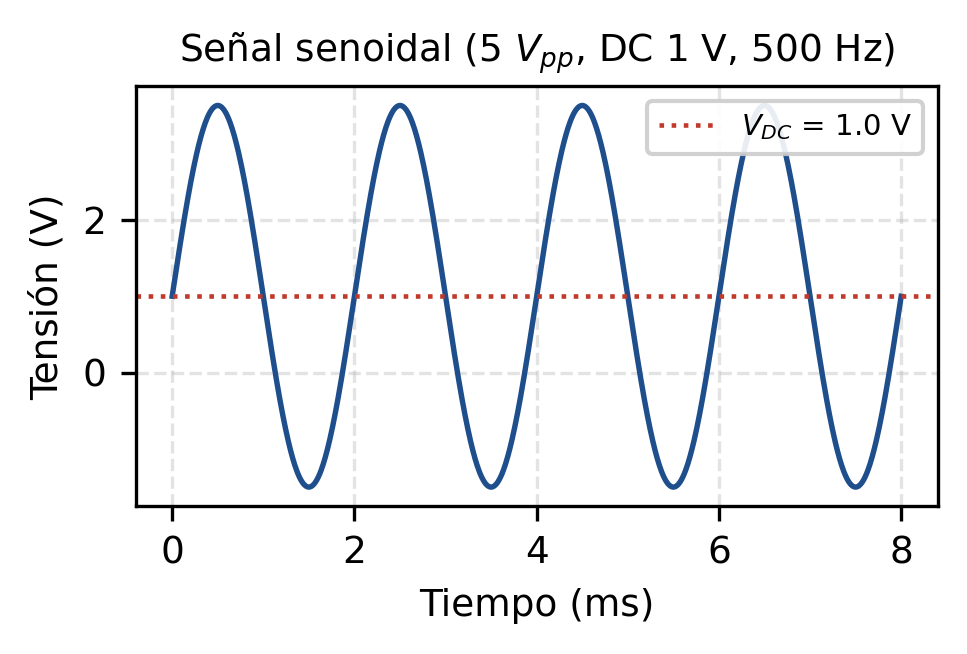
\includegraphics[width=0.48\textwidth]{grafica_senoidal.png}
    \caption{Señal senoidal simulada ($5\text{ V}_{pp}$, DC $1\text{ V}$, $500\text{ Hz}$).}
    \label{fig:sen}
\end{figure}

En la Fig. \ref{fig:cuad_sim} es posible observar la onda cuadrada simétrica manteniendo la excursión de voltaje teórica.

\begin{figure}[htbp]
    \centering
    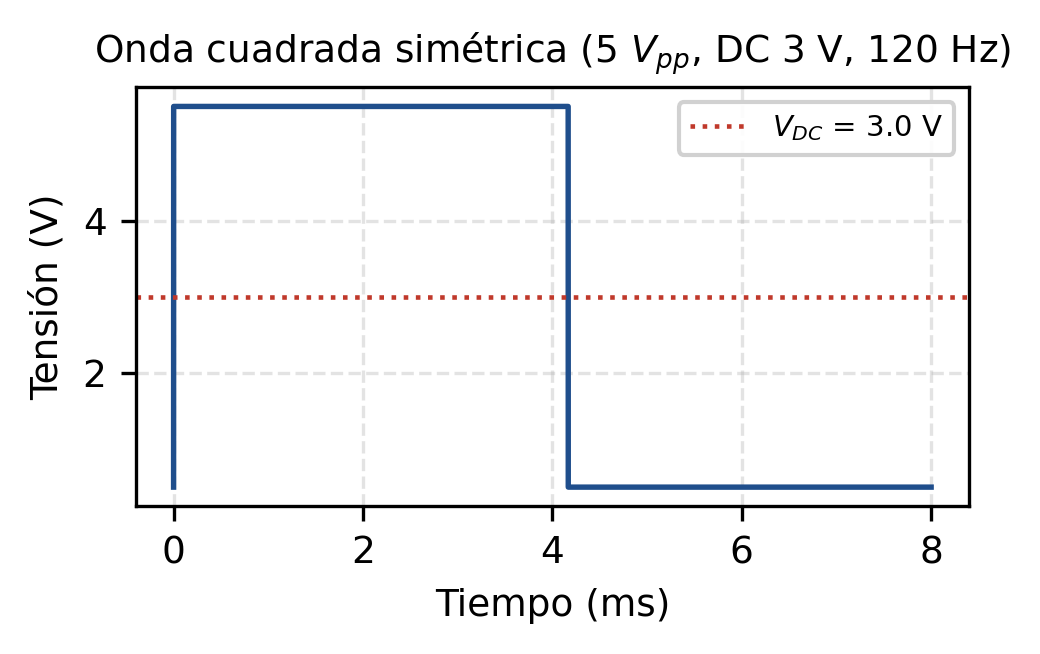
\includegraphics[width=0.48\textwidth]{grafica_cuadrada_sim.png}
    \caption{Onda cuadrada simétrica simulada ($5\text{ V}_{pp}$, DC $3\text{ V}$, $120\text{ Hz}$).}
    \label{fig:cuad_sim}
\end{figure}

En la Fig. \ref{fig:triang} es posible observar el comportamiento de la onda triangular con su respectivo offset negativo.

\begin{figure}[htbp]
    \centering
    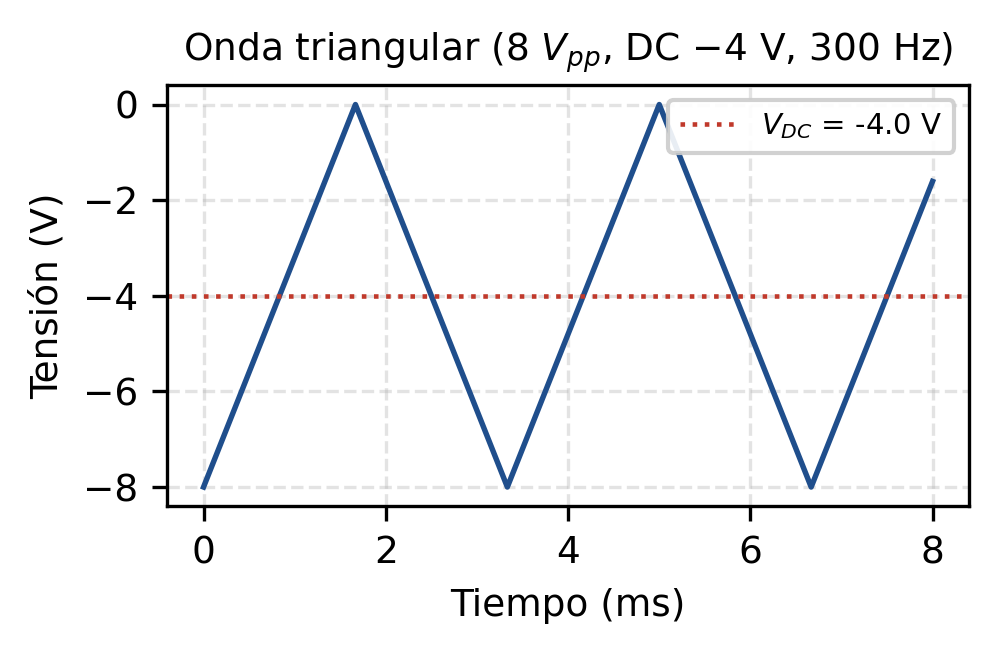
\includegraphics[width=0.48\textwidth]{grafica_triangular.png}
    \caption{Onda triangular simulada ($8\text{ V}_{pp}$, DC $-4\text{ V}$, $300\text{ Hz}$).}
    \label{fig:triang}
\end{figure}

En la Fig. \ref{fig:cuad_asim} es posible observar la onda cuadrada asimétrica con su ciclo útil del 70\%.

\begin{figure}[htbp]
    \centering
    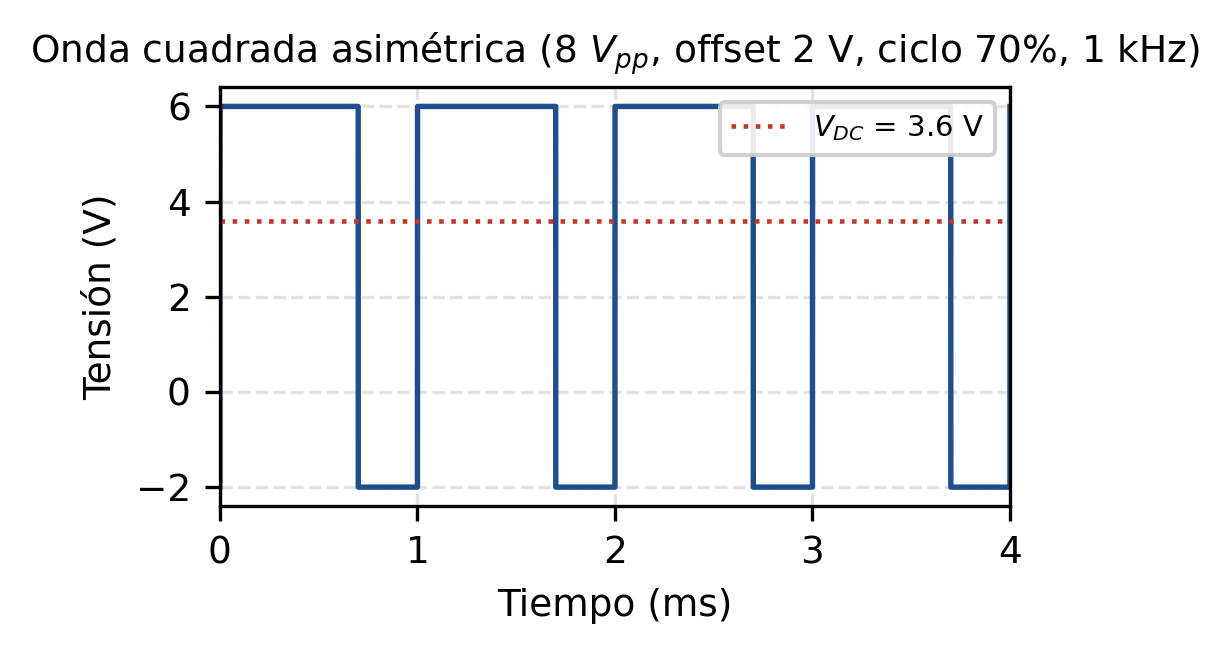
\includegraphics[width=0.48\textwidth]{grafica_cuadrada_asim.png}
    \caption{Onda cuadrada asimétrica simulada ($8\text{ V}_{pp}$, offset $2\text{ V}$, ciclo útil 70\%, $1\text{ kHz}$).}
    \label{fig:cuad_asim}
\end{figure}

A partir de estas mediciones obtenidas en el simulador, se construye la Tabla \ref{tab:senales}, que compara los resultados medidos con los teóricos.

\begin{table}[htbp]
\centering
\caption{Comparación de señales: valor teórico vs. simulado}
\label{tab:senales}
\begin{tabular}{@{}lcc@{}}
\toprule
\textbf{Señal} & \textbf{DC (Teó. / Sim.)} & \textbf{RMS (Teó. / Sim.)} \\ \midrule
Senoidal $5\text{V}_{pp}$       & 1.000 / 1.000 V   & 2.031 / 2.031 V \\
Cuadrada $5\text{V}_{pp}$       & 3.000 / 3.000 V   & 3.905 / 3.905 V \\
Triang. $8\text{V}_{pp}$        & -4.000 / -3.999 V & 4.619 / 4.618 V \\
Cuadrada asim. $8\text{V}_{pp}$ & 3.600 / 3.600 V   & 5.138 / 5.138 V \\ \bottomrule
\end{tabular}
\end{table}

\subsection{Análisis de resultados de simulacion}
En la Tabla \ref{tab:potencias} es posible observar que la mayor potencia se disipa en $R_1$, al conducir la corriente total; en contraste, $R_4$ disipa la menor potencia. En la Tabla \ref{tab:senales} es posible observar que el error entre valores teóricos y simulados es prácticamente nulo.

Respuestas a la Sección 4 de la guía \cite{guia_practica0}:

\textbf{1) Multímetros:} Un multímetro \emph{promedio} rectifica la señal y multiplica el valor medio por un factor de forma (1.11), siendo correcto solo para señales senoidales puras \cite{fluke_truerms,keysight_truerms}. Un multímetro \emph{True RMS} digitaliza la señal, eleva al cuadrado cada muestra, promedia y extrae la raíz cuadrada, entregando el valor eficaz real de cualquier forma de onda \cite{fluke_truerms}.

\textbf{2) Variables medibles:} El osciloscopio permite observar la señal en el tiempo y medir amplitud pico a pico, periodo, frecuencia y nivel DC \cite{sedra2020}. El multímetro entrega valores integrados (RMS, DC, corriente) pero no visualiza la onda \cite{sedra2020}.

\textbf{3) Límite de frecuencia:} Se debe a la capacitancia parásita en las puntas y la etapa de entrada, que forma un filtro pasa-bajos que atenúa las componentes de alta frecuencia \cite{allaboutcircuits_freqlimit}.

\textbf{4) Precisión vertical del osciloscopio:} Depende de la resolución en bits del ADC interno y del nivel de ruido propio del amplificador de entrada (\emph{front-end}), ya que el ruido degrada la resolución vertical efectiva \cite{keysight_vertacc}.

\textbf{5) Impedancias:} La impedancia de entrada representa la oposición al recibir una señal (debe ser alta para no cargar el circuito) \cite{buadlab_impedance}. La impedancia de salida es la resistencia interna de la fuente; debe ser baja para transferir la mayor tensión posible a la carga \cite{buadlab_impedance}.

\subsubsection{Observaciones finales de la simulación}
\begin{itemize}
    \item Los cálculos analíticos presentaron un margen de error casi nulo respecto al modelo simulado en SPICE, verificando el cumplimiento de las Leyes de Kirchhoff y Ohm.
    \item Las fórmulas generalistas de RMS no son aplicables a ondas cuadradas o asimétricas; se debe recurrir a la definición integral, la cual coincidió con el valor de $5.138\text{ V}$ obtenido en el simulador.
    \item Conocer la arquitectura interna de los equipos de medición permite anticipar los límites de validez de una medición y evitar errores al trabajar con señales de alta frecuencia.
\end{itemize}
\section{Montajes experimentales}
\subsection{Montaje del circuito resistivo DC}
Este circuito se construyo siguiendo las indicaciones de la guía de laboratorio. 
Se encuentra compuesto de la siguiente topología:

\begin{figure}[htbp]
    \centering
    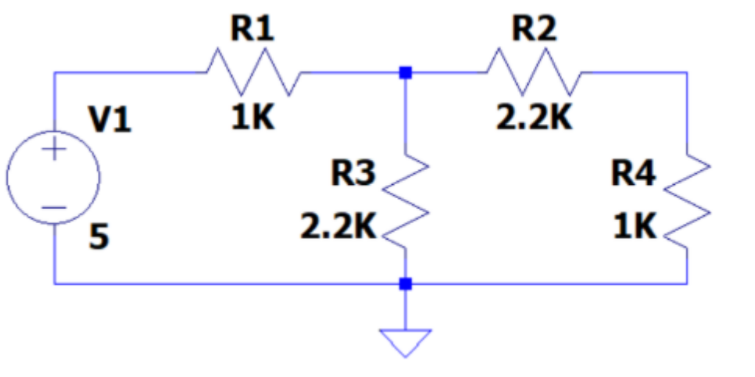
\includegraphics[width=0.48\textwidth]{circuito_1.png}
    \caption{Circuito resistivo DC \cite{guia_practica0}}
    \label{fig:circuito_1}
\end{figure}
Para la construcción de este circuito se emplearon resistencias de 1/4 de Watt con $10\%$ de tolerancia
y la fuente DC disponible en el laboratorio.
\\ por su parte para las mediciones se emplearon como voltímetro un multímetro \textit{Fluke 73} disponible en el laboratorio
y como amperímetro un multímetro \textit{FNIRSI DMT-99} el cual fue llevado por un miembro del equipo.
Ambos multímetros ajustan automáticamente la escala de medición, y dado que no se esperaban corrientes superiores a $1A$ para 
ninguna de las resistencias, el amperímetro se conecto en la escala de medición de corriente de menor tope.
\\ Con la intención de hacer las medidas lo más coherentes posibles, tanto las mediciones de tensión como de corriente para cada resistencia se realizaron de manera simultánea,
empleando sondas de aguja para el voltímetro, y cables banana-caimán para permitir el paso de corriente por el amperímetro, 
desconectando cada resistencia de su correspondiente línea en la protoboard cada que fuera necesario.

\subsection{Medición del valor RMS para distintas formas de onda}
Para las mediciones de las distintas formas de onda simuladas, simplemente se conectaron 
en paralelo los multímetros \textit{Fluke 73} de respuesta promedio, el multímetro \textit{Fluke 112} True RMS, 
y el osciloscopio \textit{Rigol DHO812} configurado para indicar también el valor RMS total. Estos equipos
medían de manera simultánea la salida del generador de ondas disponible en el laboratorio modelo \textit{Rigol DG4062}.

\begin{figure}[htbp]
    \centering
    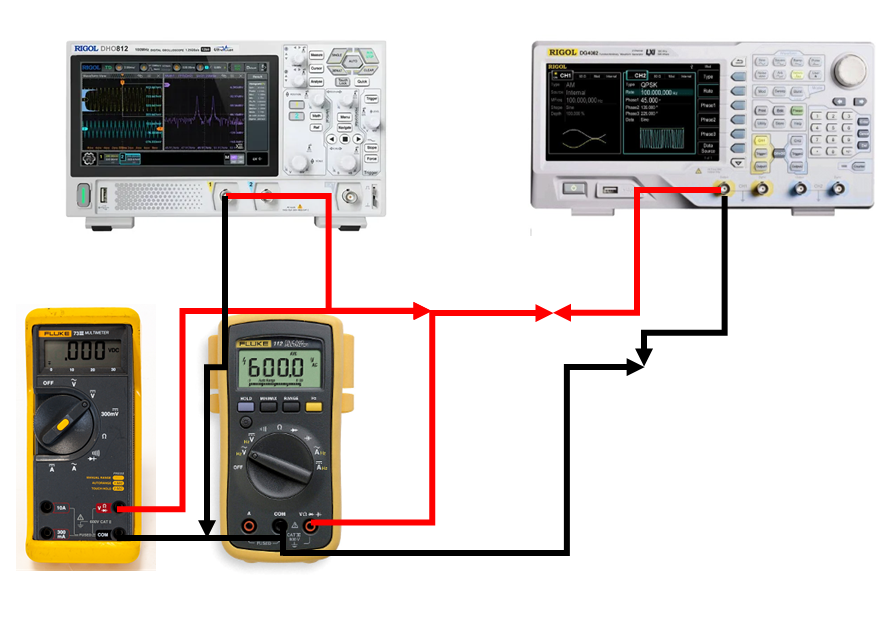
\includegraphics[width=0.48\textwidth]{circuito_2.png}
    \caption{Ilustración de conexiones realizadas para el experimento}
    \label{fig:circuito_2}
\end{figure}

\subsection{Medición de la impedancia de los equipos disponibles en el laboratorio}
Para la medición de la impedancia de los equipos presentes en el laboratorio, los equipos objetivo de la medición
fueron el generador \textit{Rigol DG4062} y el osciloscopio \textit{Rigol DHO812}.
Tal y como se describe en la guía, en los circuitos descritos se emplearon trimmers con la intención de obtener un ajuste fino, 
dado que estos circuitos se basan en la construcción de un divisor de tensión para determinar la impedancia interna de los equipos.
Para el experimento referente al generador de ondas, se empleó un trimmer de referencia \textit{ W102} de $1k\Omega$, mientras que para construir el circuito
orientado a la medición del osciloscopio, se emplearon 2 trimmers \textit{W205} de $2M \Omega$ conectados en serie.
\begin{figure}[htbp]
    \centering
    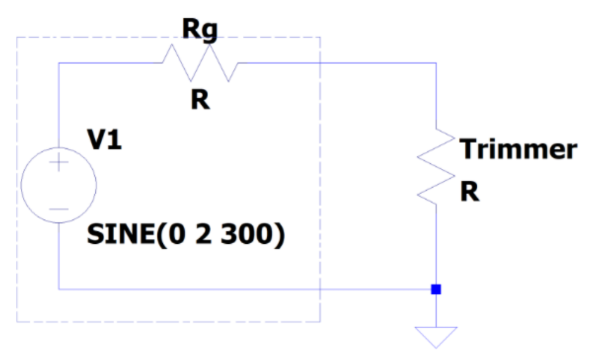
\includegraphics[width=0.48\textwidth]{generador.png}
    \caption{Esquema del circuito para la medición de la impedancia del generador de ondas\cite{guia_practica0}}
    \label{fig:impedancia_generador}
\end{figure}
\begin{figure}[htbp]
    \centering
    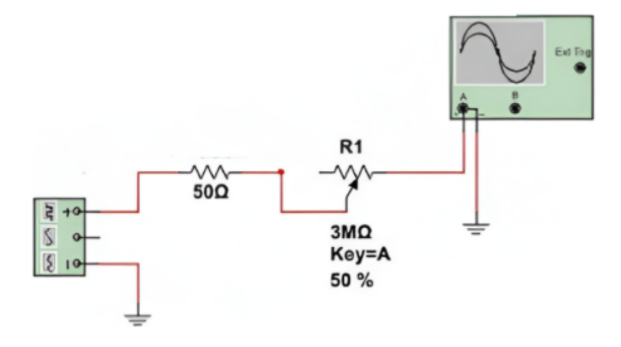
\includegraphics[width=0.48\textwidth]{osciloscopio.png}
    \caption{Esquema del circuito para la medición de la impedancia de entrada del osciloscopio \cite{guia_practica0}}
    \label{fig:impedancia_osciloscopio}
\end{figure}




\section{resultados}
A continuación se presentan los distintos valores tomados 
para cada experimento, 
\begin{table}[H]
\centering
\caption{Mediciones experimentales del circuito resistivo DC}
\label{tab:mediciones_dc}
\begin{tabular}{@{}ccccc@{}}
\toprule
  & R1     & R2    & R3     & R4     \\ \midrule
V & 2.1 V  & 1.96V & 2.84V  & 0.87V  \\
I & 2.18mA & 0.9mA & 1.31mA & 0.91mA \\ \bottomrule
\end{tabular}
\end{table}

\begin{table}[H]
\centering
\caption{Mediciones experimentales de valor RMS para distintas formas de onda}
\label{tab:mediciones_rms}
\resizebox{\columnwidth}{!}{%
\begin{tabular}{@{}cccc@{}}
\hline
\begin{tabular}[c]{@{}c@{}}Onda\end{tabular} & \multicolumn{1}{c}{\begin{tabular}[c]{@{}c@{}}Valor multímetro \\ TRMS\end{tabular}} & \multicolumn{1}{c}{\begin{tabular}[c]{@{}c@{}}Valor multímetro \\ de respuesta promedio\end{tabular}} & \multicolumn{1}{c}{\begin{tabular}[c]{@{}c@{}}Valor \\ osciloscopio\end{tabular}} \\ \hline
\begin{tabular}[c]{@{}c@{}}Seno  $5V_{pp}$ \\ + 1 VDC  500Hz\end{tabular}                          & 1.725 V                                                                              & 1.728 V                                                                                               & 1.97 V                                                                            \\ \hline
\begin{tabular}[c]{@{}c@{}}Cuadrada  $5V_{pp}$ \\ + 3V DC  120Hz\end{tabular}                      & 2.485V                                                                               & 2.759 V                                                                                               & 3.80 V                                                                            \\ \hline
\begin{tabular}[c]{@{}c@{}}Triangular  $8V_{pp}$ \\ - 4V DC  300Hz\end{tabular}                    & 2.303 V                                                                              & 2.226 V                                                                                               & 4.64 V                                                                            \\ \hline
\begin{tabular}[c]{@{}c@{}}Cuadrada \\ 70\% Duty Cycle  \\ $8V_{pp}$ \\ + 2V DC  1kHz\end{tabular} & 3.501 V                                                                              & 4 V                                                                                                   & 5.109 V                                                                           \\ \hline
\end{tabular}%
}
\end{table}
\subsection{Impedancias de los equipos}
\section{análisis de resultados}



\renewcommand{\refname}{Referencias}
\begin{thebibliography}{99}
\bibitem{guia_practica0} Universidad Nacional de Colombia, ``Práctica 0: Manejo de Equipos,'' Guía de Laboratorio, Electrónica Análoga I, 2026.
\bibitem{sedra2020} A. S. Sedra, et al., \textit{Microelectronic Circuits}, 8th ed. Oxford University Press, 2020.
\bibitem{militaryaerospace_scopes} J. Paul, ``The significance of oscilloscopes in aerospace and defense,'' \textit{Military Aerospace Electronics}.
\bibitem{pilotjohn_scopes} PilotJohn, ``Oscilloscopes -- Aircraft Electrical System Analysis.''
\bibitem{tektronix_biomedical} Tektronix, ``Making MicroVolt Biomedical Measurements.''
\bibitem{fluke_truerms} Fluke Corporation, ``When Do You Actually Need a True-RMS Multimeter?''
\bibitem{keysight_truerms} Keysight Technologies, ``Tip 1: Understand True RMS Measurements.''
\bibitem{allaboutcircuits_freqlimit} All About Circuits Forum, ``Digital/Analog Multimeter, Frequency Limit in AC reading.''
\bibitem{keysight_vertacc} Keysight Technologies, ``Why is Oscilloscope Vertical Accuracy Important?''
\bibitem{buadlab_impedance} Boston University, ``Input and output impedance.''
\end{thebibliography}

\end{document}